% mnras_template.tex
%
% LaTeX template for creating an MNRAS paper
%
% v3.0 released 14 May 2015
% (version numbers match those of mnras.cls)
%
% Copyright (C) Royal Astronomical Society 2015
% Authors:
% Keith T. Smith (Royal Astronomical Society)

% Change log
%
% v3.0 May 2015
%    Renamed to match the new package name
%    Version number matches mnras.cls
%    A few minor tweaks to wording
% v1.0 September 2013
%    Beta testing only - never publicly released
%    First version: a simple (ish) template for creating an MNRAS paper

%%%%%%%%%%%%%%%%%%%%%%%%%%%%%%%%%%%%%%%%%%%%%%%%%%
% Basic setup. Most papers should leave these options alone.
%\documentclass[onecolumn,a4paper,fleqn,usenatbib]{mnras}
\documentclass[a4paper,fleqn,usenatbib]{mnras}

% MNRAS is set in Times font. If you don't have this installed (most LaTeX
% installations will be fine) or prefer the old Computer Modern fonts, comment
% out the following line
\usepackage{newtxtext,newtxmath}
% Depending on your LaTeX fonts installation, you might get better results with one of these:
%\usepackage{mathptmx}
%\usepackage{txfonts}

% Use vector fonts, so it zooms properly in on-screen viewing software
% Don't change these lines unless you know what you are doing
\usepackage[T1]{fontenc}
\usepackage{ae,aecompl}

%%%%% AUTHORS - PLACE YOUR OWN PACKAGES HERE %%%%%

% Only include extra packages if you really need them. Common packages are:
\usepackage{graphicx}	% Including figure files
\usepackage{amsmath}	% Advanced maths commands
\usepackage{amssymb}	% Extra maths symbols
\usepackage[xindy]{glossaries}
\glsdisablehyper
\usepackage{subcaption}
\captionsetup{compatibility=false}

%%%%%%%%%%%%%%%%%%%%%%%%%%%%%%%%%%%%%%%%%%%%%%%%%%

%%%%% AUTHORS - PLACE YOUR OWN COMMANDS HERE %%%%%

% Please keep new commands to a minimum, and use \newcommand not \def to avoid
% overwriting existing commands. Example:
%\newcommand{\pcm}{\,cm$^{-2}$}	% per cm-squared

\newcommand{\GSF}[1]{\noindent\textcolor{blue}{GSF:#1}}

%glossary
\newacronym{alfa}{ALFA}{Arecibo L-Band Feed Array}
\newacronym{dm}{DM}{Dispersion Measure}
\newacronym{frb}{FRB}{Fast Radio Burst}
\newacronym{fwhm}{FWHM}{Full-Width at Half-Maximum}
\newacronym{gbt}{GBT}{Greenbank Telescope}
\newacronym{if}{IF}{Intermediate Frequency}
\newacronym{igm}{IGM}{Intergalactic Medium}
\newacronym{ism}{ISM}{Interstellar Medium}
\newacronym{lo}{LO}{Local Oscillator}
\newacronym{nip}{NIP}{Non-image Processing}
\newacronym{pll}{PLL}{Phased-locked Loop}
\newacronym{rfi}{RFI}{Radio-frequency Interference}
\newacronym{ska}{SKA}{Square Kilometre Array}
\newacronym{sefd}{SEFD}{System Equivalent Flux Density}
\newacronym{snr}{SNR}{Signal-to-Noise Ratio}
\newacronym{sps}{SPS}{Single Pulse Search}

%%%%%%%%%%%%%%%%%%%%%%%%%%%%%%%%%%%%%%%%%%%%%%%%%%

% Title of the paper, and the short title which is used in the headers.
% Keep the title short and informative.
\title[Verification Tests for FRB Detections]{Verification Tests for FRB
Detections}

\author[ALFABURST Team]{
ALFABURST Team
}
%% The list of authors, and the short list which is used in the headers.
%% If you need two or more lines of authors, add an extra line using \newauthor
%\author[K. T. Smith et al.]{
%Keith T. Smith,$^{1}$\thanks{E-mail: mn@ras.org.uk (KTS)}
%A. N. Other,$^{2}$
%Third Author$^{2,3}$
%and Fourth Author$^{3}$
%\\
%% List of institutions
%$^{1}$Royal Astronomical Society, Burlington House, Piccadilly, London W1J 0BQ, UK\\
%$^{2}$Department, Institution, Street Address, City Postal Code, Country\\
%$^{3}$Another Department, Different Institution, Street Address, City Postal Code, Country
%}

% These dates will be filled out by the publisher
\date{Accepted XXX. Received YYY; in original ZZZ}

% Enter the current year, for the copyright statements etc.
\pubyear{2017}

% Don't change these lines
\begin{document}
\label{firstpage}
\pagerange{\pageref{firstpage}--\pageref{lastpage}}
\maketitle

% Abstract of the paper
\begin{abstract}
% What is the point of the paper?
% What is the context of the study? What background information is necessary to understand the study?
% How was the study done?
% What is the main take away message?
% What can be said about these results, and how does this affect future work?
The one-off nature of most Fast Radio Bursts (FRBs) requires extra scrutiny in
reporting an astrophysical FRB and triggering automated follow-ups with a
telescope network.  The ALFABURST commensal FRB survey at Arecibo Observatory
has been in operation since June 2015. In that time a number of false-positive
events, which on initial inspect appear to be FRB-like, have been found to be of
local origin. Here we report on one such event as an example of the difficult
challenge of fully automating an FRB search. We discuss observational and
post-processing techniques which are useful to further automate an FRB search
survey.
\end{abstract}

% Select between one and six entries from the list of approved keywords.
% Don't make up new ones.
\begin{keywords}
radio continuum: transients -- methods: observational
\end{keywords}

%%%%%%%%%%%%%%%%% BODY OF PAPER %%%%%%%%%%%%%%%%%%

\section{Introduction}
\label{sec:intro}

In the two years of the initial ALFABURST survey\citep{2017ApJS..228...21C} over
125k 8-second windows have been recorded in which our \gls{frb} search pipeline
detected an event above the minimum \gls{snr} detection threshold. The vast
majority of these events have been due to \gls{rfi}, some of the events are due
to bright single pulses of known pulsars. Sorting through these false positive
events is the main focus of our post-processing methods. Most of the events are
clearly \gls{rfi} which are classified with an automated classifier model. A
small number of windows contain FRB-like events which only on further inspection
of the data, the telescope operation status, and contextual information is it
clear that these events are from local sources.

We expect a number of false-positives to pass our post-processing detection
tests, as we would like to severely limit the potential for type-II errors in our
classifier by accepting a number of type-I errors. So far, all false-positives
we have detected are explainable as relating to the telescope or \gls{rfi} by
examining the observing situation after the fact. This creates a challenge of
automating the triggering of follow-up signalling to other telescopes. Either
there will be an excess of false-positive triggers but with a short delay
between detection and triggering. Or, a non-automated, expert examination of the
event is required to verify, creating a delay in any follow-up.

In this letter, we report on FRB-like signals detected with our ALFABURST system,
and discuss how we have improved our post-processing pipeline and observing
system to handle unexpected, but explainable signals. These improvements are
valuable to incorporate into any \gls{frb} search survey.

\section{An example of a FRB-like Signal detected with ALFABURST}
\label{sec:D20161204}

A narrow-in-time, broad-in-frequency, millisecond pulse was detected with the
ALFABURST system at MJD 57726.563263913 / Unix time 1480858266 (09:31:06 Arecibo
local time) in Beam 0 (the central beam) of the \gls{alfa}
receiver\footnote{http://www.naic.edu/alfa/} (Figure
\ref{fig:beam0_dynamic_spec}). ALFABURST was processing 56 MHz of bandwidth
between 1457 MHz and 1513 MHz. The \gls{snr} of this pulse is maximized (10.46)
when the pulse is dedispersed with a \gls{dm} of 293 and the 256 microsecond
resolution is decimated by a factor of 16 to 4 ms time resolution. The
dedispered time series shows an approximately 20 ms \gls{fwhm} pulse. The dip
before and after the pulse is due to the DM-zero removal (i.e. the moving
average is subtracted) during pulse detection. This is a simple way to remove a
drifting gain baseline at the cost of removing some of the overall pulse power,
particularly at low DM. The bright, narrow-band signal at approximately $t=0.1$
seconds is locally generated \gls{rfi} which we will cover later in this
section.

\begin{figure*}
    \centering
    % notebooks/ALFABURST_events.ipynb
    \begin{subfigure}[t]{0.45\textwidth}
        \centering\captionsetup{width=.95\linewidth}
        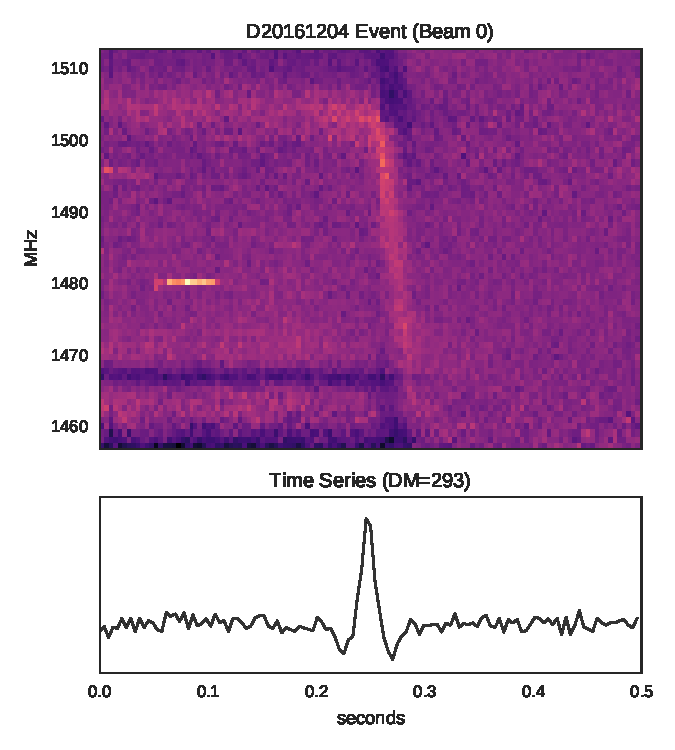
\includegraphics[width=1.0\textwidth]{figures/D20161204_buf23_Beam0.pdf}
        \caption{Detected FRB-like event in beam 0 of ALFA. The characteristic dip
        before and after the event is due to zero-DM removal which is part of the
        ALFABURST RFI exciser. The strong, narrowband source at 1480 MHz around 0.1
        s is due to a  local RFI source.  }
        \label{fig:beam0_dynamic_spec}
    \end{subfigure}
    % notebooks/ALFABURST_events.ipynb
    \begin{subfigure}[t]{0.45\textwidth}
        \centering\captionsetup{width=.95\linewidth}
        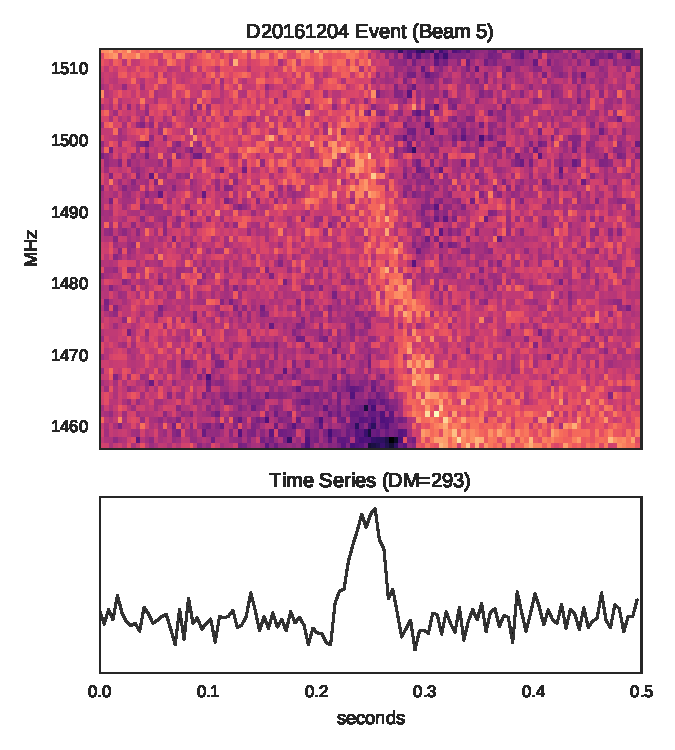
\includegraphics[width=1.0\textwidth]{figures/D20161204_buf4_Beam5.pdf}
        \caption{Detected FRB-like event in beam 5 of ALFA. The event width
        appears wider than the beam 0 event as the zero-DM dips are not as
        prominent.
        }
        \label{fig:beam5_dynamic_spec}
    \end{subfigure}
    \caption{
    Dynamic spectrum (top) and dedispersed time series (bottom) of an FRB-like
    event that was detected simultaneously in beam 0 and 5 of the ALFA receiver
    on December 4, 2016. The dynamic spectrum has been bandpass normalized.
    }
    \label{fig:dynamic_spec}
\end{figure*}

On initial inspection, this event looks like a promising new astrophysical
\gls{frb}. The flux density of the event can be computed with the radiometer
equation
%
$$
S = \textrm{SEFD} \frac{\textrm{SNR}}{\sqrt{D \; \Delta \tau \;
\Delta \nu}}
$$
%
using a \gls{sefd} of 3 Jy for the \gls{alfa} receiver. This results in a flux
density of $S = 66$ mJy from Beam 0, which would be lower flux than any
previously detected \gls{frb} \citep{2016PASA...33...45P}. This flux estimate is
a lower limit, as we are assuming the source was at the centre of the beam. The
width is on the high end for \glspl{frb} but still within the range of those
previously reported.

We inspected all other events in the same time window as the Beam 0 event. An
event was found in Beam 5 only (Figure \ref{fig:beam5_dynamic_spec}). This pulse
lines up exactly in time with the Beam 0 event but the \gls{frb} was maximized
(15.99) with a DM=829 dedispersion. Upon further inspection and testing
different DMs for dedispersion we found that this event appeared to narrow in
width at lower DM trials. We see that there was \gls{rfi} clipping in this event
which is known to introduce a bias, resulting in a maximized \gls{snr} at a
different DM trial. The beam 0 and beam 5 event are the same event.

The beam 5 detection has a lower \gls{snr} than the beam 0 detection at DM trial
293. This is still reasonable as the beam 0 side-lobes overlap with all the other
beams, as does the beam 5 side-lobe overlap with the beam 0 primary beam. This
would indicate that the sky source is somewhere between the beam 0 and beam 5
pointing centres. And, the detection was from the edge of the primary lobe or in
the side-lobe of each beam.

The width of the dedispersed pulse in beam 5 appears wider, but this is likely
due to the lower \gls{snr} of the event having a smaller effect on the
spectrum normalization.

One can look at the immediate period before and after the pulse to see that
there are no similar events (Figure \ref{fig:dm_time}). The event appears to be
isolated in time, with a fairly compact representation in DM-space. The event
would be detected with significant \gls{snr} at higher \gls{dm} trials due to
the wide width of the pulse, but peaks at a \gls{dm} trial of 293.

% notebooks/ALFABURST_events.ipynb
%\begin{figure}
%    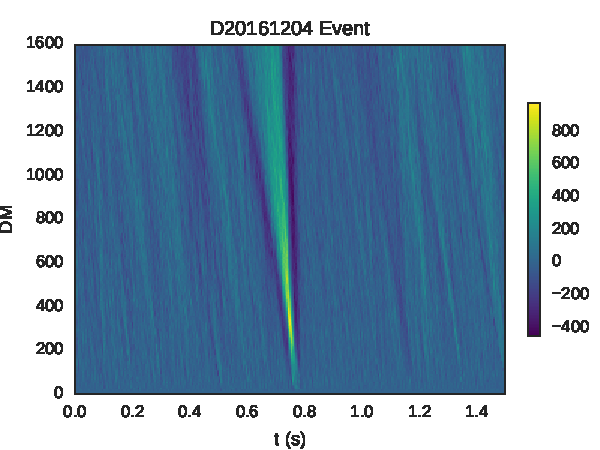
\includegraphics[width=1.0\linewidth]{figures/D20161204_dmtrials_buf23_Beam0.pdf}
%    \caption{DM vs. time plot of for a 1.5 second window centred on the December
%    4th event in beam 0. The SNR peaks at a DM of 293. There is a significant
%    detection at larger DM trials due to the width of the pulse.
%    }
%    \label{fig:dm_time}
%\end{figure}
%
\begin{figure}
    \centering
    % notebooks/ALFABURST_events.ipynb
    \begin{subfigure}[t]{0.5\textwidth}
        \centering\captionsetup{width=.95\linewidth}
        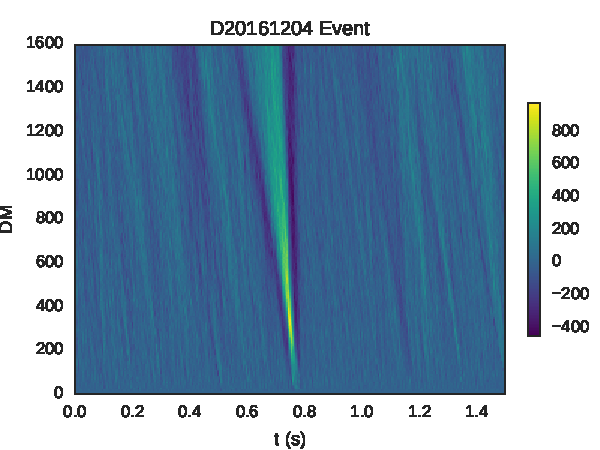
\includegraphics[width=1.0\textwidth]{figures/D20161204_dmtrials_buf23_Beam0.pdf}
        \caption{DM vs. time plot of for a 1.5 second window centred on the December
        4th event in beam 0. The SNR peaks at a DM of 293. There is a significant
        detection at larger DM trials due to the width of the pulse.
        }
        \label{fig:dm_time_event}
    \end{subfigure}
    % notebooks/ALFABURST_events.ipynb
    \begin{subfigure}[t]{0.5\textwidth}
        \centering\captionsetup{width=.95\linewidth}
        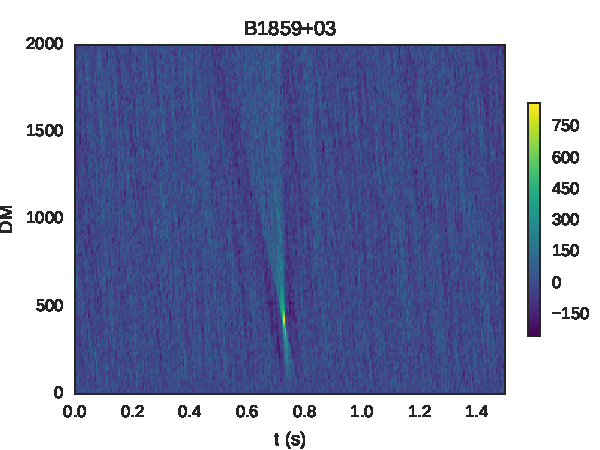
\includegraphics[width=1.0\textwidth]{figures/B1859_dmtrials.pdf}
        \caption{DM vs. time plot of a brigth single pulse from B1859+03 which
        has a DM of 402 and pulse width of 11 ms (W50).
        }
        \label{fig:dm_time_B1859}
    \end{subfigure}
    \caption{DM-space plot shows the characteristic butterfly pattern of the
    narrow-in-time, dispersed pulse detected by ALFABURST. A single pulse
    detection of B1859+03 is shown for reference.
    }
    \label{fig:dm_time}
\end{figure}

The Arecibo telescope logging data is reported locally in SCRAM packets which
provide pointing, frequency tuning, and receiver information at approximately
one second resolution. From these logs, the telescope was pointed at a fixed Dec
(+15:11:28.34) and drifting in RA (event detected at RA=14:42:26.18), i.e. a
fixed (alt,az) pointing during the event. No known pulsar or RRAT is within the
beam at this pointing.

We considered that the observing band could have been changed in that time.  We
have setup the automated system to restart observations when the \gls{if}
frequency is changed.  During the time of the event, there was no change in the
\gls{if} during that time.

The SCRAM logs do provide the first indication that this event is due to a local
source. Beyond the pointing and \gls{if}, the SCRAM logs report the position of
the receiver turret and if \gls{alfa} is active. \gls{alfa} is at a position
angle of approximately $26.64^{\circ}$ in the turret, the system reported the
turret was at $206^{\circ}$. \gls{alfa} is not in, or even near the focus.  Our
commensal observation script checks if \gls{alfa} is active before we run
ALFABURST. This is a check on whether the analogue receiver chain is properly
setup for \gls{alfa}, which almost always means that \gls{alfa} is in the focus.
But, as we have found out, there are times when this is not true.

The SCRAM logs do not report the active project or observing schedule. During
the time of the event it appears that no receiver was in use, otherwise,
\gls{alfa} would not have been active, and we see that \gls{alfa} was
deactivated approximately 20 minutes after the event when a new observation
began.  Looking at the observation schedule for the morning of December 4,
project
P3080\footnote{http://www.naic.edu/vscience/schedule/tpfiles/MichillitagP3080tp.pdf}
was using \gls{alfa} to perform an \gls{frb} survey of the Virgo cluster until
09:00 local time.  After 09:00 local time Project
R3037\footnote{http://www.naic.edu/vscience/schedule/tpfiles/TaylortagR3037tp.pdf}
was scheduled, this is an S-Band RADAR observation. 

Looking at the average bandpass of beam 0 and 5 during the time of the event, we
see that the shape and system noise appear different to what is expected during
typical observations (Figure \ref{fig:bandpass_response}).  The detection band
of \gls{alfa} was chosen because it is the most sensitive region of the band,
and relatively flat. But during the event, there is a noticeable shape and slant
to the bandpass which is different than the typical bandpass.  Beam 0 and 5
bandpasses look related in elements of their bandpass shape, and the narrow-band
features due to the short, bright \gls{rfi} events that occur during the
recorded time window. The system noise appears to be higher during the event,
which leads to the bandpasses appearing smoother than the typical bandpass.  In
the detection pipeline the data is normalized, so all absolute scaling is
removed in the process. This indicates that the \gls{sefd} is too low in our
flux calibration. This increase is system noise is due to the change in turret
position, and the \gls{alfa} feed picking up reflections from other equipment in
the dome, and the dome as a warm source.

% notebooks/ALFABURST_events.ipynb
\begin{figure}
    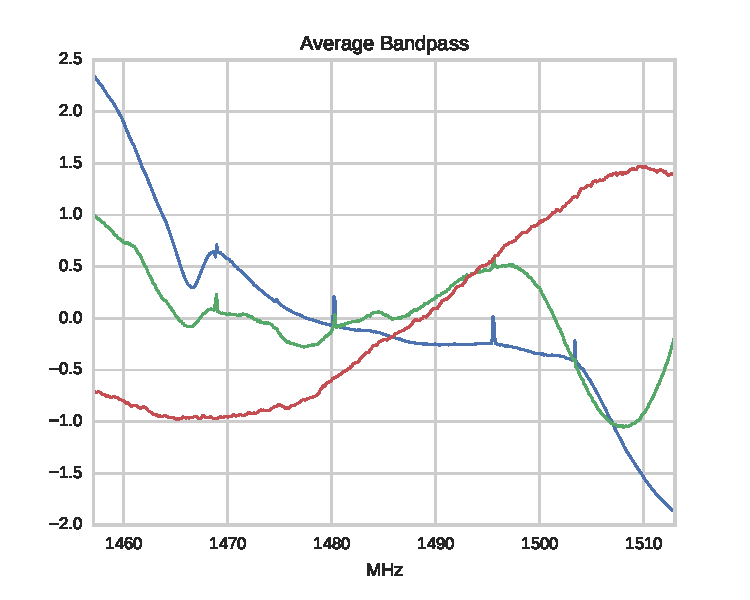
\includegraphics[width=1.0\linewidth]{figures/bandpass_response.pdf}
    \caption{Average bandpass response during the December 4, 2016 event for beam
    0 (green) and beam 5 (blue). A typical bandpass (red) is plotted for
    reference. These bandpasses have been normalized in the detection pipeline.
    }
    \label{fig:bandpass_response}
\end{figure}

We then looked at previously recorded events close in time to the event.
Approximately 80 seconds earlier another window was recorded which has large
structures across the band (Figure \ref{fig:beam0_dynamic_spec_80s}). Though not
as narrow in time as the event, they appear related to the same phenomenon.

The DM - time plot (Figure \ref{fig:beam0_dmtrials_80s}) shows that much of the
structure would be detected as dispersed pulses.  In particular, the structure
around 4 seconds would be detected as a wide-in-time, highly dispersed pulse.
And the structure immediately proceeding it would be detected as a negative
dispersed pulse.  We do not detect these as pulses because we have limited our
search space to narrow-in-time width pulses and positive \glspl{dm}. Our choice
of search space is reasonable for the type of events we wish to detect given
limited computing resources. But, there are practical advantages to searching
negative \glspl{dm} and wider-in-time pulse widths. We expect astrophysical
pulses to have positive \glspl{dm}. But, system variation and \gls{rfi} can
produce signals which result in positive and negative \gls{dm} detections.  A
statistical measure can be made in any time window to differentiate times of
significant, but low-level \gls{rfi} or system variation from actual
astrophysical pulses. Testing out to larger pulse widths is computationally
cheap as the time window is decimated, reducing the memory usage. A full sampling
of larger pulse widths or negative \gls{dm} trials like the positive \gls{dm}
trials is not necessary. Only a subset can be computed to provide a useful
information on the stability of the system and \gls{rfi} environment.

\begin{figure*}
    \centering
    % notebooks/ALFABURST_events.ipynb
    \begin{subfigure}[t]{1.0\textwidth}
        \centering\captionsetup{width=.95\linewidth}
        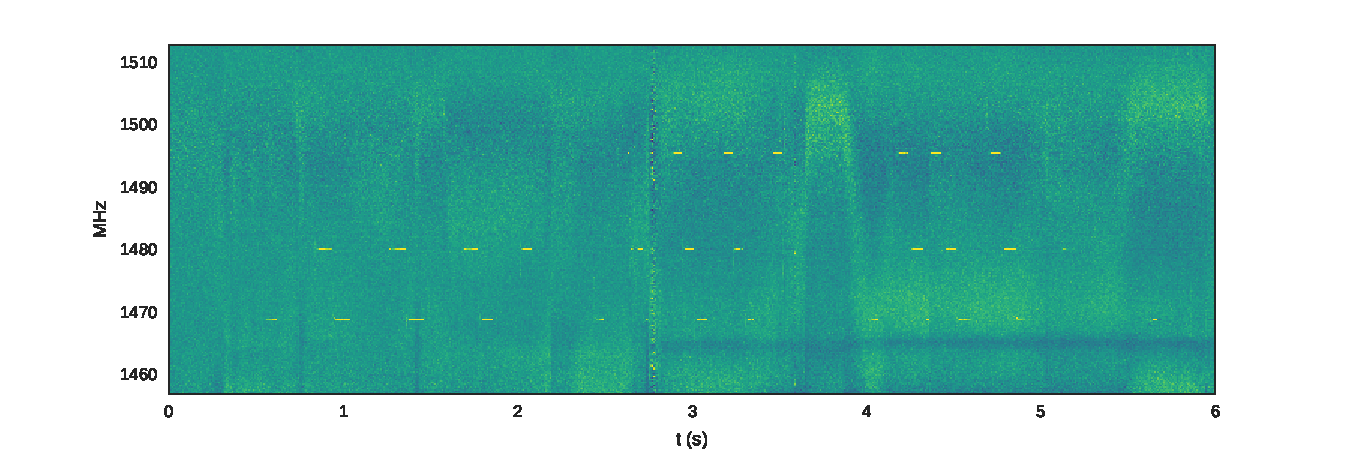
\includegraphics[width=1.0\textwidth]{figures/D20161204_spect_buf21_Beam0.pdf}
        \caption{Dynamic spectrum shows frequency evolution of the bandpass as a
        function of time with structures similar to the D20161204 event.
        }
        \label{fig:beam0_dynamic_spec_80s}
    \end{subfigure}
    % notebooks/ALFABURST_events.ipynb
    \begin{subfigure}[t]{1.0\textwidth}
        \centering\captionsetup{width=.95\linewidth}
        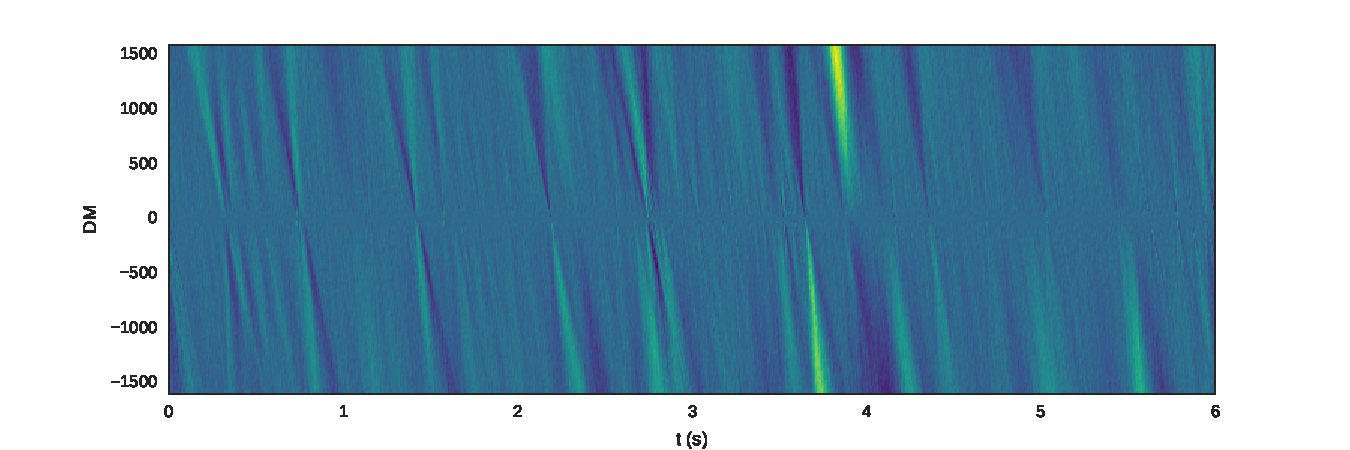
\includegraphics[width=1.0\textwidth]{figures/D20161204_dmtrials_buf21_Beam0.pdf}
        \caption{DM trials from -1600 to 1600 show that there would be both
        positive and negative pulse detections during this time window.
        }
        \label{fig:beam0_dmtrials_80s}
    \end{subfigure}
    \caption{Dynamic spectrum (top) and DM-time plot (bottom) of 6 seconds from
    beam 0 approximately 80 seconds before the D20161204 event.
    }
    \label{fig:beamo0_80s}
\end{figure*}

The narrow-in-frequency, periodic RFI at 1468, 1480, 1496,
1504 MHz is not usually seen in this band. In the high time and frequency
resolution view these short pulses in 12.5 MHz steps have a characteristic
dampened harmonic oscillation due to frequency locking with a \gls{pll} (Figure
\ref{fig:pll_spectrum}). With help from the Arecibo Observatory staff, this has
been identified as an instrumentational \gls{rfi} from an instrument that is
routinely used to monitor the local \gls{rfi} environment.
%
% notebooks/ALFABURST_events.ipynb
\begin{figure}
    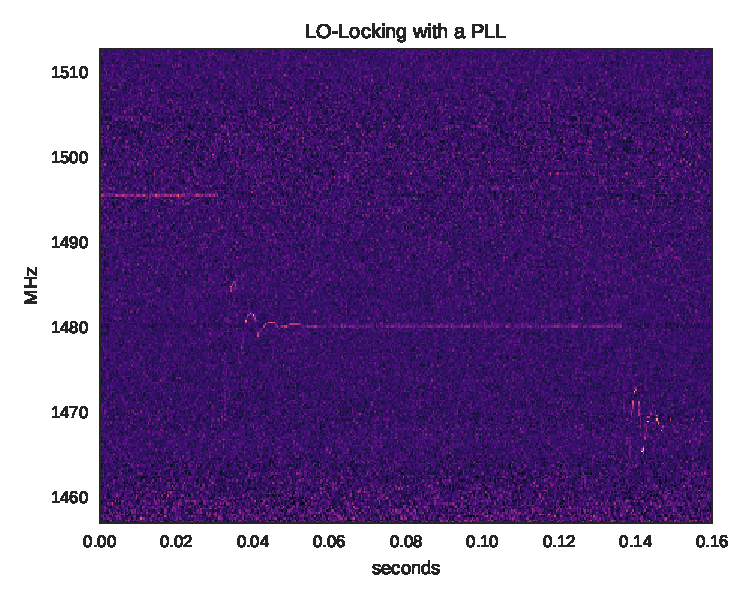
\includegraphics[width=1.0\linewidth]{figures/pll_spectrum.pdf}
    \caption{Dynamic spectrum when a local oscillator in the receiver dome is
    being locked with a phase-locked loop circuit. This LO is not related to
    the receiver analogue mixing chain, but rather it is associated with RFI
    monitoring equipment.
    }
    \label{fig:pll_spectrum}
\end{figure}
%
The exact physical process which generated these apparently dispersed pulses is
not perfectly well known. But, the picture is that the \gls{alfa} receiver was
out of the main focus, likely picking up reflections from the dome, leading to
an increase in the system temperature. An \gls{rfi} monitoring program was being
run on an instrument not included in the telescope SCRAM data. This instrument
introduced the narrowband \gls{rfi} due to changing of a \gls{lo}, and possibly
the broadband \gls{rfi}. With high certainty, we can classify this as a local
event which created the appearance of an \gls{frb}.  In isolation, and the
one-off, transient nature of FRBs make the initial Beam 0 detection look very
reasonable. It is only with an extended study of the meta-data, earlier-in-time
evolution of the band, and use of multiple beams to confirm that this is indeed
not an FRB of astronomical origin.

\section{Low-SNR False-Positive Detections}
\label{sec:low_snr}

% TODO:
% low SNR events, due to sudden changes in the noise statistics, expect to
% detect a few of these based in the minimum SNR, what is the time scale for an
% SNR 6 event? these events are due to turrent movement, add flag to filter out
% figure: DM - t plot

% TODO: mention that multiple promising events have been detected with Arecibo,
% only after follow-up was it clear that the detection was due to a local
% effect.

\section{Detected RADAR Event with ARTEMIS}
\label{sec:LOFAR_RADAR}

ARTEMIS \citep{2015MNRAS.452.1254K} is a similar to ALFABURST \gls{frb} search
survey run at the LOFAR-UK station at Chilbolton Observatory. The ARTEMIS survey
uses a similar fractional bandwidth ($\sim 0.04$) to the ALFABURST survey, but
centred around 145 MHz. This survey is setup to have known pulsars regularly
transit the fixed in local coordinate beams. Single pulses are routinely
detected. Occasionally, \gls{rfi} events are detected by the automated pipeline. 
A particularly interesting event was detected which had a maximized \gls{snr}
with a \gls{dm} of 85 is shown in Figure \ref{fig:lofar_dynamic}. The
narrow-in-time pulse can be seen in the dynamic spectrum at frequencies above
146 MHz, but is not apparent at lower frequencies. As there is significant
narrow band \gls{rfi} below 146 MHz it could be that the pulse is buried. The
dedispered time series shows a strong detection of a pulse of approximately 20
ms in width.
%
% notebooks/LOFAR_RADAR.ipynb
\begin{figure}
    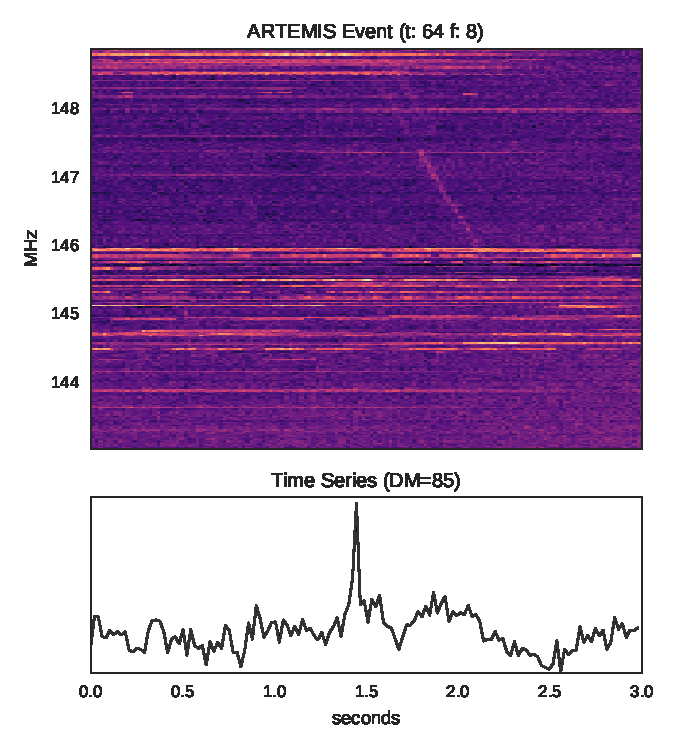
\includegraphics[width=1.0\linewidth]{figures/LOFAR_dynamic.pdf}
    \caption{A dispersed pulse detected by the automated ARTEMIS search
    pipeline. The dispresed pulse only appears over a narrow band of just over 1
    MHz.
    }
    \label{fig:lofar_dynamic}
\end{figure}
%
The celestial pointing of the beam during the time of the event is not
associated with any known pulsar or RRAT at a DM around 85. This is DM is low
compared to reported \gls{frb} detections.
% TODO: pointing, SNR, maximized DM and time decimation, NE2001 model for
% distance

Plotting the event in a DM-space across the ARTEMIS DM range (0-320) (Figure
\ref{fig:lofar_dm_time}) shows a strong, compact detection which we would expect
to see of a dispersed pulse during a time of minimal \gls{rfi}.
%
% notebooks/LOFAR_RADAR.ipynb
\begin{figure}
    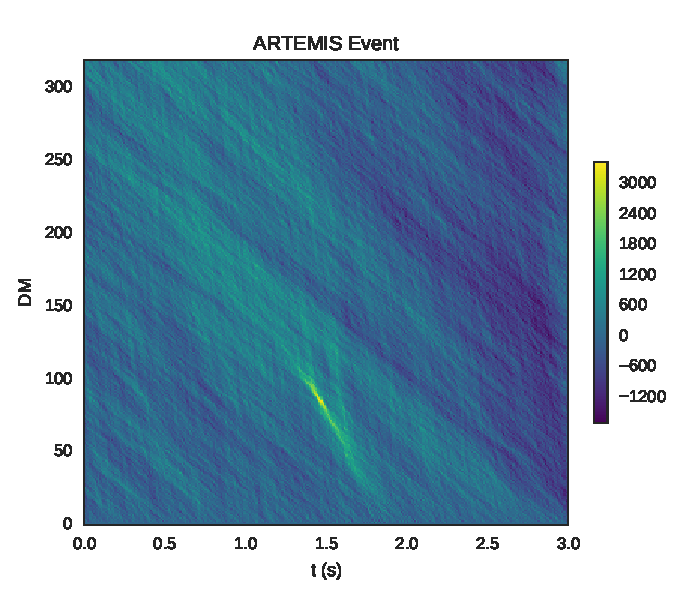
\includegraphics[width=1.0\linewidth]{figures/LOFAR_dm_time.pdf}
    \caption{DM-space plot of the event shows a strong, compact detection around
    DM=85 with no other apparent events during at the time.
    }
    \label{fig:lofar_dm_time}
\end{figure}
%
Since the pulse is only apparent in part of the band we became suspicious of its
origin. It could be that the pulse is broadband but the brightest component is
only seen in the 146-147 MHz region. Or, it could be a band-limited pulse.  The
search pipeline, like ALFABURST and many other search pipelines, decimates the
dynamic spectrum in time to search for over a range of pulse widths. In the case
of the event shown in Figure \ref{fig:lofar_dynamic} the maximized \gls{snr}
occurred with a time decimation factor of 20, the native resolution is $327.68
\mu s$, resulting in a decimated time resolution of 20 ms. By plotting the event
at a higher time resolutions (Figure \ref{fig:lofar_dynamic_high}) we can see
there is a distinct repeating pattern in time not previously apparent. This is a
linearly frequency modulated signal used for pulse compression in RADAR. In
RADAR observations the bandwidth of the transmitter provides information on the
range and direction of a target. A narrow band RADAR transmitter can be used to
approximate a larger bandwidth by modulating the frequency of the transmitted
pulse. There are a number of allocated usages in this band which could be the
source of this RADAR pulse \citep{ofcom2017}.  As the RADAR signal is a
dispersed pulse we would expect to detect such signals with ARTEMIS.
%
% notebooks/LOFAR_RADAR.ipynb
\begin{figure}
    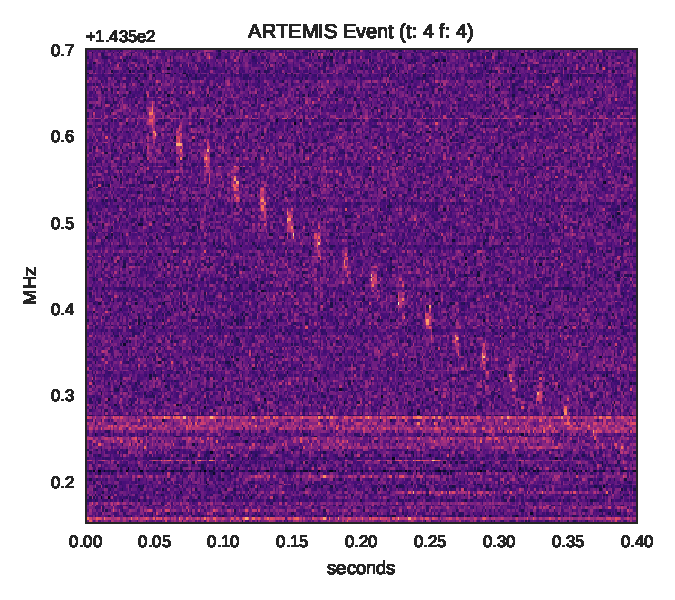
\includegraphics[width=1.0\linewidth]{figures/LOFAR_dynamic_high_res.pdf}
    \caption{A zoomed in view of the event in Figure \ref{fig:lofar_dynamic} at
    high time and frequency resolution shows the distinct pattern of a linearly frequency
    modulated RADAR pulse.
    }
    \label{fig:lofar_dynamic_high}
\end{figure}
%
Verification of this event was straight forward by examining the high-time and
frequency resolution data to see the pulsed nature of the event. The frequency
allocation and the use of standard RADAR techniques across the radio band is a
clear indicator of the origin of this event. The challenge comes in the
verification and automated signalling if the desire is to run the system in
real-time with immediate follow-up with additional telescopes. The RADAR event
occurs rarely and there is no obvious detection filter automate. Expert
knowledge in radio signals and visual acuity are necessary to make a decision
about the event. If we are willing to allow an automated VOevent trigger where
we expect a number of false-positives then we can except the rare
\gls{rfi} trigger.

\section{Verification Checks}

The one-off nature of \glspl{frb} makes it essential that when reporting on a
detection or triggering a follow-up observation that significant due-diligence
is done in order to verify a positive detection as much as possible. Over the
past decade of \gls{frb} surveys a number of techniques have been developed to
efficiently filter for dispersed pulses. The vast majority of events are flagged
by \gls{rfi} excisers and setting a sufficiently high minimum \gls{snr}
threshold. 

% TODO:
% decision tree
% important tests:
%   bandpass check
%   telescope status
%   negative DM statistics
%   previous in time events
%   high time/freq resolution dynamic spectrum
%   dm-space plot

Current surveys typically search out to extreme \glspl{dm}, in the case of
ALFABURST we search out to a \gls{dm} of 10000 as the additional computational
cost is minimum. If the \gls{dm}-redshift relation is approximately correct,
searching to such high \glspl{dm} is sufficent to sample out to the very early
universe. We expect an astrophysical source to be despersed by a positive
\gls{dm} value. As such we do not search for negatively despersed pulses. But,
\gls{rfi} does show up as both positive and negative desipersion detections
(Figure \ref{fig:beamo0_80s}). As the dedispersion search is no longer
computationally limited it would be possible to search the negative \gls{dm}
space. This would be useful as a statistical statement about the number of
positive versus negative detections to quantify the amount of \gls{rfi} during a
detection. The full negative \gls{dm} space would not need to be searched, a
regular sampling of the space would be sufficient.

% TODO: considerations for automated follow-up/VOevents

% TODO: considerations for releasing FRB event data as they are one-off events that
% require extra scrutiny

% TODO:
% future developments in FRB surveys require additional layers of processing.
% large surveys will produce an abundance of false positives. it is cumbersome
% to follow up events now. in the future it will be impossible. additional
% layers should prioritize events by how interesting they are

% TODO: FRB130729
% https://heasarc.gsfc.nasa.gov/cgi-bin/Tools/xTime/xTime.pl
% Linear Frequency Modulated Pulse Waveforms
% https://en.wikipedia.org/wiki/Pulse_compression
% http://www.radartutorial.eu/02.basics/Stepped%20Chirp%20Radar.en.html
% google: radar chirp l band, radar chirp quadratic, stepped chirp l band
% stepped chirp waveform

Jupyter notebooks and the filterbanks files are hosted on our
public git repository\footnote{https://github.com/griffinfoster/ab-survey-2017}.

\bibliographystyle{mnras}
\bibliography{../alfaburst.bib} 

% Don't change these lines
\bsp	% typesetting comment
\label{lastpage}
\end{document}

% End of mnras_template.tex
